\RequirePackage{iftex}
\ifPDFTeX
\documentclass[a4paper,12pt]{article}
\usepackage[margin=24mm]{geometry}
\usepackage[T1]{fontenc}
\usepackage[utf8]{inputenc}
\usepackage{graphicx}
\usepackage{CJKutf8}
\else
\documentclass[a4paper,12pt]{jsarticle}
\usepackage[dvipdfmx,margin=24mm]{geometry}
\usepackage[dvipdfmx]{graphicx}
\fi
\usepackage{amsmath,amssymb,amsthm}
\usepackage{enumitem}
\usepackage{tikz}
\usepackage{url}
\usetikzlibrary{arrows.meta,calc}

\setlength{\parindent}{0pt}
\setlength{\parskip}{0.35em}
\setlength{\fboxsep}{8pt}
\setlist[itemize]{leftmargin=2em,itemsep=0.25em,topsep=0.35em}

\newcommand{\feedbackqa}[2]{%
\item[]
\begin{tabular}[t]{@{}p{1.8em}@{\hspace{0.4em}}p{\dimexpr\linewidth-2.2em\relax}@{}}
Q. & #1 \\
A. & #2
\end{tabular}
\par\smallskip\hrulefill
}

\newcommand{\pointbox}[1]{%
\begin{center}
\fbox{%
\begin{minipage}{0.9\linewidth}
#1
\end{minipage}}
\end{center}
}

\begin{document}
\ifPDFTeX
\begin{CJK}{UTF8}{min}
\fi

\theoremstyle{definition}
\newtheorem*{definition}{定義}
\newtheorem*{theorem}{定理}
\newtheorem*{lemma}{補題}
\newtheorem*{corollary}{系}
\newtheorem*{example}{例}
\renewcommand{\proofname}{証明}

\begin{center}
{\LARGE 数学1A 第6回レジュメ}\\[0.4em]
テイラー展開とオイラーの公式
\end{center}
\section*{フィードバック}

\begin{itemize}[leftmargin=1.5em,itemsep=0.7em,topsep=0.3em]
\feedbackqa{授業ででてきた系とはなにか?}{系とは定理からすぐに導かれる主張をいいます。今日紹介した系は剰余項が$0$に収束すれば, テイラー展開が成立するという主張ですが、これは定理からすぐに導かれるので、定理とは呼ばずに系と呼ぶことにしました。}
\feedbackqa{系の証明の部分がよくわからなかった。}{授業では説明するのを省きましたが、
$$|a_n-a|\to 0 \Leftrightarrow \lim_{n\to\infty} a_n = a$$
という関係式を$a_n = \sum^n _{k=0} \frac{f^{(k)}(a)}{k!}(x-a)^k $, $a=f(x)$に適用してしました。}
\feedbackqa{レポートの模範解答$\varepsilon$-$\delta$の問題の$\delta$のとりかたでminという授業で扱っていないものがでてきた}{大変申し訳ありません。minは定義していませんでしたね。他の$\delta$のとり方としては
$$\delta= \frac{1}{1+(4/\varepsilon)}$$
というとり方でも証明できます}
\feedbackqa{グループワークでの図示が難しい}{７次はやりすぎましたね。中間テスト含めて今後図示させる問題は出しませんので安心してください。}
\feedbackqa{列にわりこまれて電車にすわれなかった}{大変でしたね}
\feedbackqa{グラフをどこまで正確にかけばよいか}{少なくともこの授業では、近似してるなぁという実感を持っていただければ良いので、そこまでちゃんとかける必要はないです。}
\feedbackqa{グループワークで全員に同じ問題を出してほしい}{5回に1回できたらいいなと思っています}
\feedbackqa{中島が数学を勉強していて一番楽しいと思う瞬間}{なにか新しいものを発見したときですね。オイラーの公式の1/10000くらいの重要さだとしても、新しいものを発見したときの喜びは代えがたいものです}
\feedbackqa{もう少し黒板の字を大きく書いてほしい}{承知しました。次回から気をつけます。}
\feedbackqa{テイラー定理のおすすめの勉強}{ハードルは高いですが、自分で証明をなにもみずに書いてみたり、参考書をみずに、適当な関数のテイラー展開を計算してみると良いと思います}
 
\end{itemize}

\section*{小テスト}

\begin{enumerate}[leftmargin=2em,itemsep=0.5em,topsep=0.3em]
\item $f(x)=\cos x$ の $a=\frac{\pi}{2}$ における $1$ 次，$3$ 次のテイラー多項式を求め，図示せよ。
\item $T_n(x)=\sum_{j=0}^{n}\frac{f^{(j)}(a)}{j!}(x-a)^j$ とする。$0\leq k\leq n$ に対して，$T_n^{(k)}(x)$ と $T_n^{(k)}(a)$ を求めよ。
\end{enumerate}

\subsection*{答え}

\begin{enumerate}[leftmargin=2em,itemsep=0.7em,topsep=0.3em]
\item $h=x-\frac{\pi}{2}$ とおくと，$\cos x=\cos\left(\frac{\pi}{2}+h\right)=-\sin h$ である。したがって
\[
T_1(x)=-\left(x-\frac{\pi}{2}\right),
\qquad
T_3(x)=-\left(x-\frac{\pi}{2}\right)+\frac{1}{6}\left(x-\frac{\pi}{2}\right)^3.
\]

\begin{center}
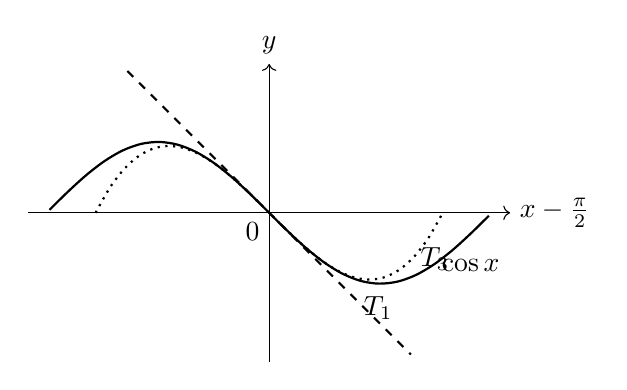
\begin{tikzpicture}[scale=0.9]
\draw[->] (-3.4,0)--(3.4,0) node[right] {$x-\frac{\pi}{2}$};
\draw[->] (0,-2.1)--(0,2.1) node[above] {$y$};
\draw[domain=-3.1:3.1,smooth,variable=\u,thick] plot ({\u},{-sin(\u r)});
\draw[domain=-2.0:2.0,smooth,variable=\u,dashed,thick] plot ({\u},{-\u});
\draw[domain=-2.45:2.45,smooth,variable=\u,dotted,thick] plot ({\u},{-\u+\u*\u*\u/6});
\node[right] at (2.3,-0.75) {$\cos x$};
\node[right] at (1.2,-1.35) {$T_1$};
\node[right] at (2.0,-0.65) {$T_3$};
\node[below left] at (0,0) {$0$};
\end{tikzpicture}
\end{center}

\item $T_n(x)$ を $k$ 回微分すると
\[
T_n^{(k)}(x)
=\sum_{j=k}^{n}\frac{f^{(j)}(a)}{(j-k)!}(x-a)^{j-k}
\]
である。特に $x=a$ を代入すると，$j=k$ の項だけが残るので
\[
T_n^{(k)}(a)=f^{(k)}(a)
\]
である。
\end{enumerate}

\section{テイラーの定理}

前回，$f$ の $a$ における $n$ 次テイラー多項式を
\[
T_n(x)=\sum_{k=0}^{n}\frac{f^{(k)}(a)}{k!}(x-a)^k
\]
と定義した。テイラーの定理は，この多項式がどれくらい $f(x)$ を近似しているかを教えてくれる。

\begin{theorem}[テイラーの定理]
$I$ を区間とし，$a,x\in I$ とする。$f$ が $a$ と $x$ の間で $n+1$ 回連続的微分可能であるとき，ある $\xi$ が $a$ と $x$ の間に存在して
\[
f(x)=T_n(x)+\frac{f^{(n+1)}(\xi)}{(n+1)!}(x-a)^{n+1}
\]
が成り立つ。
\end{theorem}
\begin{proof}
$x=a$ のときは等式は明らかである。以下 $x\neq a$ とする。
\[
P(t)=\sum_{k=0}^{n}\frac{f^{(k)}(a)}{k!}(t-a)^k
\]
とおき，
\[
F(t)=f(t)-P(t),\qquad G(t)=(t-a)^{n+1}
\]
とする。$P$ は $f$ の $a$ における $n$ 次テイラー多項式なので，
\[
F(a)=F'(a)=\cdots=F^{(n)}(a)=0
\]
が成り立つ。また $G(a)=G'(a)=\cdots=G^{(n)}(a)=0$ である。

まず $F$ と $G$ にコーシーの平均値の定理を用いると，$a$ と $x$ の間にある点 $c_1$ が存在して
\[
\frac{F(x)-F(a)}{G(x)-G(a)}=\frac{F'(c_1)}{G'(c_1)}
\]
となる。左辺は $\frac{F(x)}{G(x)}$ である。次に $F'$ と $G'$ にコーシーの平均値の定理を用いると，$a$ と $c_1$ の間にある点 $c_2$ が存在して
\[
\frac{F'(c_1)-F'(a)}{G'(c_1)-G'(a)}
=\frac{F''(c_2)}{G''(c_2)}
\]
となる。左辺は $\frac{F'(c_1)}{G'(c_1)}$ である。

同じ議論を繰り返すと，ある $\xi$ が $a$ と $x$ の間に存在して
\[
\frac{F(x)}{G(x)}=\frac{F^{(n+1)}(\xi)}{G^{(n+1)}(\xi)}
\]
となる。ここで $P^{(n+1)}(t)=0$ かつ $G^{(n+1)}(t)=(n+1)!$ なので
\[
\frac{f(x)-P(x)}{(x-a)^{n+1}}
=\frac{f^{(n+1)}(\xi)}{(n+1)!}
\]
である。したがって
\[
f(x)=P(x)+\frac{f^{(n+1)}(\xi)}{(n+1)!}(x-a)^{n+1}
\]
である。
\end{proof}

\begin{lemma}
任意の実数 $x$ に対して
\[
\frac{x^n}{n!}\to 0 \quad (n\to\infty)
\]
が成り立つ。
\end{lemma}
\begin{proof}
$x=0$ のときは明らかである。以下 $x\neq 0$ とする。
$N\in \mathbb{N}$ を $N>|x|$ となるようにとる。このとき $n\geq 2N+1$ ならば
\[
\frac{|x|^n}{n!}
=\frac{|x|}{1}\cdot \frac{|x|}{2}\cdots \frac{|x|}{n}
\leq
\left(\frac{|x|}{1}\cdots \frac{|x|}{N}\right)
\left(\frac{|x|}{N+1}\cdots \frac{|x|}{n}\right).
\]
ここで $N>|x|$ なので，$j\geq N+1$ ならば $\frac{|x|}{j}\leq \frac{N}{N+1}<1$ である。したがって
\[
0\leq \frac{|x|^n}{n!}
\leq
\left(\frac{|x|}{1}\cdots \frac{|x|}{N}\right)
\left(\frac{N}{N+1}\right)^{n-N}
\]
となる。右辺は $n\to\infty$ で $0$ に収束するので，
\[
\frac{|x|^n}{n!}\to 0
\]
である。よって $\frac{x^n}{n!}\to 0$ も成り立つ。
\end{proof}
\begin{corollary}
テイラーの定理における $c=c(x,n)$ について，
\[
\lim_{n\to\infty}\frac{f^{(n+1)}(c)}{(n+1)!}(x-a)^{n+1}=0
\]
が成り立つならば，
\[
f(x)=\sum_{k=0}^{\infty}\frac{f^{(k)}(a)}{k!}(x-a)^k
\]
が成り立つ。
\end{corollary}
\begin{proof}
テイラーの定理と仮定より
\[
\left|f(x)-T_n(x)\right|
=\left|\frac{f^{(n+1)}(c)}{(n+1)!}(x-a)^{n+1}\right|
\to 0.
\]
したがって
\[
\sum_{k=0}^{\infty}\frac{f^{(k)}(a)}{k!}(x-a)^k
=\lim_{n\to\infty}T_n(x)=f(x)
\]
である。
\end{proof}
\section{$e^x$ のテイラー展開}

\begin{theorem}
任意の実数 $x$ に対して
\[
e^x=\sum_{k=0}^{\infty}\frac{x^k}{k!}
\]
が成り立つ。
\end{theorem}

\begin{proof}
$f(x)=e^x$ とし，$a=0$ で考える。すべての $k$ に対して $f^{(k)}(x)=e^x$ だから
\[
T_n(x)=\sum_{k=0}^{n}\frac{x^k}{k!}
\]
である。また，$0$ と $x$ の間の任意の $c$ に対して $e^c\leq e^{|x|}$ なので
\[
\left|\frac{f^{(n+1)}(c)}{(n+1)!}x^{n+1}\right|
\leq e^{|x|}\frac{|x|^{n+1}}{(n+1)!}\to 0
\]
である。したがって系より
\[
e^x=\sum_{k=0}^{\infty}\frac{x^k}{k!}
\]
である。
\end{proof}

\section{$\sin x$ と $\cos x$ のテイラー展開}

\begin{theorem}
任意の実数 $x$ に対して
\[
\sin x=\sum_{k=0}^{\infty}(-1)^k\frac{x^{2k+1}}{(2k+1)!},
\qquad
\cos x=\sum_{k=0}^{\infty}(-1)^k\frac{x^{2k}}{(2k)!}
\]
が成り立つ。
\end{theorem}

\begin{proof}
$f(t)=\sin t$ について考える。導関数は
\[
\sin t,\quad \cos t,\quad -\sin t,\quad -\cos t,\quad \sin t,\dots
\]
と周期的に変わる。$x=0$ を代入すると
\[
f^{(2k)}(0)=0,\qquad f^{(2k+1)}(0)=(-1)^k
\]
となる。したがって
\[
T_n(x)=\sum_{0\leq 2k+1\leq n}(-1)^k\frac{x^{2k+1}}{(2k+1)!}
\]
である。
また，$\sin x$ のどの階の導関数も絶対値は $1$ 以下である。したがって，$0$ と $x$ の間の任意の $c$ に対して
\[
 \left|\frac{f^{(n+1)}(c)}{(n+1)!}x^{n+1}\right|
 \leq \frac{|x|^{n+1}}{(n+1)!}\to 0
\]
である。系より
\[
\sin x=\sum_{k=0}^{\infty}(-1)^k\frac{x^{2k+1}}{(2k+1)!}
\]
である。

$g(t)=\cos t$ についても同様に考える。導関数は
\[
\cos t,\quad -\sin t,\quad -\cos t,\quad \sin t,\quad \cos t,\dots
\]
と周期的に変わる。$x=0$ を代入すると
\[
g^{(2k+1)}(0)=0,\qquad g^{(2k)}(0)=(-1)^k
\]
となる。剰余項も同じく
\[
 \left|\frac{g^{(n+1)}(c)}{(n+1)!}x^{n+1}\right|
 \leq \frac{|x|^{n+1}}{(n+1)!}\to 0
\]
である。系より
\[
\cos x=\sum_{k=0}^{\infty}(-1)^k\frac{x^{2k}}{(2k)!}
\]
である。
\end{proof}

\section{オイラーの公式}

複素数 $z$ に対して，指数関数を
\[
e^z=\sum_{k=0}^{\infty}\frac{z^k}{k!}
\]
で定義する。この定義は，実数 $z=x$ のときには先ほどの $e^x$ のテイラー展開と一致する。

\begin{theorem}[オイラーの公式]
任意の実数 $x$ に対して
\[
e^{ix}=\cos x+i\sin x
\]
が成り立つ。
\end{theorem}

\begin{proof}
指数関数のテイラー展開に $z=ix$ を代入すると
\[
e^{ix}=\sum_{n=0}^{\infty}\frac{(ix)^n}{n!}
\]
である。偶数次と奇数次に分けると
\[
e^{ix}
=\sum_{k=0}^{\infty}\frac{(ix)^{2k}}{(2k)!}
+\sum_{k=0}^{\infty}\frac{(ix)^{2k+1}}{(2k+1)!}.
\]
ここで $i^{2k}=(-1)^k$，$i^{2k+1}=i(-1)^k$ なので
\[
e^{ix}
=\sum_{k=0}^{\infty}(-1)^k\frac{x^{2k}}{(2k)!}
+i\sum_{k=0}^{\infty}(-1)^k\frac{x^{2k+1}}{(2k+1)!}.
\]
右辺の実部は $\cos x$，虚部は $\sin x$ である。したがって
\[
e^{ix}=\cos x+i\sin x
\]
を得る。
\end{proof}

\section{オイラーの公式の応用}

\subsection*{三角関数の加法定理}

指数関数の性質 $e^{i(x+y)}=e^{ix}e^{iy}$ とオイラーの公式を用いると
\[
\cos(x+y)+i\sin(x+y)
=(\cos x+i\sin x)(\cos y+i\sin y)
\]
である。右辺を展開すると
\[
(\cos x\cos y-\sin x\sin y)
+i(\sin x\cos y+\cos x\sin y)
\]
となる。実部と虚部を比較して
\[
\cos(x+y)=\cos x\cos y-\sin x\sin y,
\]
\[
\sin(x+y)=\sin x\cos y+\cos x\sin y
\]
を得る。

\subsection*{差の公式}

加法定理で $y$ を $-y$ に置き換えると
\[
\cos(x-y)=\cos x\cos y+\sin x\sin y,
\]
\[
\sin(x-y)=\sin x\cos y-\cos x\sin y
\]
となる。

\subsection*{二倍角の公式}

加法定理で $y=x$ とすると
\[
\cos(2x)=\cos^2 x-\sin^2 x,
\]
\[
\sin(2x)=2\sin x\cos x
\]
を得る。また，$\cos^2 x+\sin^2 x=1$ を使えば
\[
\cos(2x)=2\cos^2 x-1=1-2\sin^2 x
\]
とも書ける。

\subsection*{ド・モアブルの公式}

$n$ を整数とする。オイラーの公式より
\[
(\cos x+i\sin x)^n=(e^{ix})^n=e^{inx}
\]
である。再びオイラーの公式を用いると
\[
e^{inx}=\cos(nx)+i\sin(nx)
\]
なので
\[
(\cos x+i\sin x)^n=\cos(nx)+i\sin(nx)
\]
を得る。

\subsection*{基本恒等式}

オイラーの公式で $x$ と $-x$ を考えると
\[
e^{ix}e^{-ix}=1
\]
であり，一方で
\[
(\cos x+i\sin x)(\cos x-i\sin x)=\cos^2 x+\sin^2 x
\]
である。したがって
\[
\cos^2 x+\sin^2 x=1
\]
が従う。

\ifPDFTeX
\end{CJK}
\fi

\end{document}
